\subsection{Context Switching}
\label{sec:registers}

Application software targeting the 64-bit Intel architecture uses a variety of
CPU registers to interact with the processor's features. The values in these
registers make up an application's state, or context. Kernels multiplex a
CPU\footnote{Actually, each hardware thread is multiplexed among software
threads. See \S~\ref{sec:cpu_core}.}
among multiple software threads by \textit{context switching}, namely saving a
thread's context, and replacing it with another thread's previously saved
context. This section covers the context switching features used by SGX when a
logical processor starts or stops executing code that belongs to an enclave.

\begin{figure}[hbt]
  \center{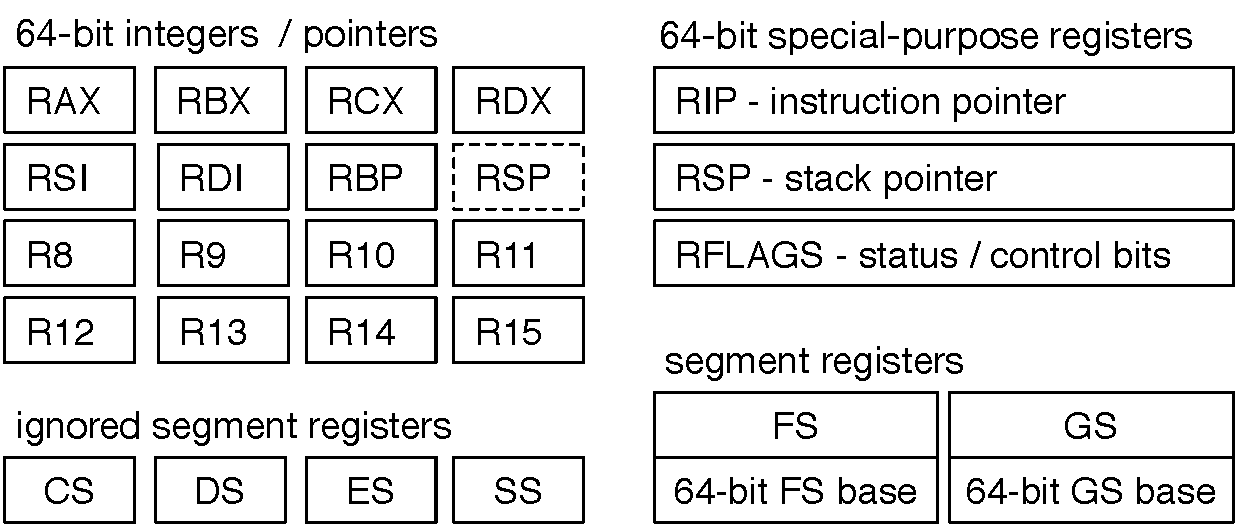
\includegraphics[width=85mm]{figures/cpu_registers.pdf}}
  \caption{
    CPU registers in the 64-bit Intel architecture. RSP can be used as a
    general-purpose register (GPR), e.g., in pointer arithmetic, but it always
    points to the top of the program's stack. Segment registers are covered in
    \S~\ref{sec:segments}.
  }
  \label{fig:cpu_registers}
\end{figure}

Integers and memory addresses are stored in 16 \textit{general-purpose
registers} (GPRs). RAX, RBX, RCX, RDX, RSI, RDI, RSP, and RBP are extended
versions of the GPRs available to 32-bit programs, and R9-R16 are new
registers. RSP is reserved for pointing to the top of the \textit{stack}, which
is automatically read and modified by the CPU instructions for procedure calls,
(e.g., CALL and RET), and by explicit stack handling instructions such as PUSH
and POP.

All applications also use the RIP register, which contains the address of the
currently executing instruction, and the RFLAGS register, whose bits (e.g.,
the carry flag - CF) are individually used to store comparison results and
control various instructions.

Software might use other registers to interact with specific features, some of
which are shown in Table~\ref{fig:xsave_state}.

\begin{table}[hbt]
  \center{\begin{tabularx}{\columnwidth}{| l | X | l |}
  \hline
  \textbf{Feature} & \textbf{Registers} & \textbf{XCR0 bit}\\
  \hline
  FPU & FP0 - FP7, FSW, FTW & 0 \\
  \hline
  SSE & MM0 - MM7, XMM0 - XMM15, XMCSR & 1 \\
  \hline
  AVX & YMM0 - YMM15 & 2 \\
  \hline
  \end{tabularx}}
  \caption{Sample feature-specific Intel architecture registers.}
  \label{fig:xsave_state}
\end{table}

The Intel architecture provides a future-proof method for an OS kernel to save
the values of feature-specific registers used by an application. The XSAVE
instruction takes in a bitmap of features, and writes the registers used by
the features whose bits are set to 1 in a memory area that can be used by the
XRESTORE instruction to load the saved values back into feature-specific
registers.

Application software declares the features that it plans to use to the kernel,
so the kernel knows what XSAVE bitmap to use when context-switching. When
receiving the system call, the kernel sets the XCR0 register to the feature
bitmap declared by the application. The CPU generates a fault if application
software attempts to use features that are not enabled by XCR0, so applications
cannot modify feature-specific registers that the kernel wouldn't take into
account when context-switching. The kernel can use the CPUID instruction to
learn the size of the XSAVE memory area for a given feature bitmap, and compute
how much memory it needs to allocate for the context of each of the
application's threads.
